
\chapter{Pruebas de funcionamiento}

Para revisar el buen funcionamiento de la aplicación desarrollada, se utilizaró el software dispuesto por Apple Inc,  el entorno de desarrollo Xcode y herramientas asociadas. Para obtener estas aplicaciones, es necesario poseer una cuenta de desarrollador para \textbf{iOS} o \textbf{Mac OS X}, las cuales se pueden obtener en el sitio web \url{https://developer.apple.com/programs/} luego de pagar la matrícula impuesta.\\

La cuenta de desarrollador permite acceso al repositorio de herramientas \cite{apple-repositorio} y también acceso a versiones de los sistemas operativos antes de lanzamiento.
Además permite poner a la venta las aplicaciones desarrolladas en la \textit{\textbf{App Store}}\cite{apple-appstore}.

% datos en el camino, seguimiento de un tweet, pantallazos de debug
\section{Cambio de tiempo y/o canal}

Las primeras pruebas estuvieron relacionadas con el cambio de tiempo a través de peticiones al dispatcher con argumentos en la cadena de consulta, estas se realizaron con la aplicación de OS X: \textbf{Quicktime X}, la cual permite reproducir streams que cumplen con las espeficicaciones de HTTP Live Streaming. Otra alternativa que además se encuentra disponible en otros sistemas operativos es \textbf{VideoLan VLC}. Las pruebas consistieron en modificar los argumentos \textbf{t}, \textbf{s} y \textbf{c} de URLs del tipo:
\url{http://ssdemo.altavoz.net/playlist/playlist.m3u8?s=tvn&t=1353186024&c=0}, donde el parámetro \textbf{t} corresponde al tiempo Unix del 17 de noviembre de 2012 18:00:24 GMT-3.\\

El escificar el tiempo en el parámetro \textbf{t} resulta siempre en una lista de reproducción con segmentos asociados al tiempo correspondiente. Además se monitoreó la respuesta a través de la aplicación rastreadora de paquetes Wireshark. Para esto se necesitó aplicar un filtro especial de forma que los paquetes relacionados con HTTP Live Streaming fueran entregados. El filtro corresponde a mostrar paquetes recibidos desde el servidor donde el cliente, en este caso Quicktime, se contacta para obtener una lista de reproducción, y además pedir la entrega de paquetes que tengan en su contenido la palabra \textbf{apple}.

\begin{figure}[H]
	\centering
\begin{lstlisting}
		ip.addr==200.91.44.49 && http contains apple
\end{lstlisting}
\caption{Filtro en Wireshark que muestra sólo paquetes relacionados con el HLS}
\end{figure}


Los resultados obtenidos son los esperados y corresponden a la reproducción del video en el momento indicado y en el canal indicado según los parámetros.

\begin{figure}[H]
	\centering
	\begin{tabular}{cc}
	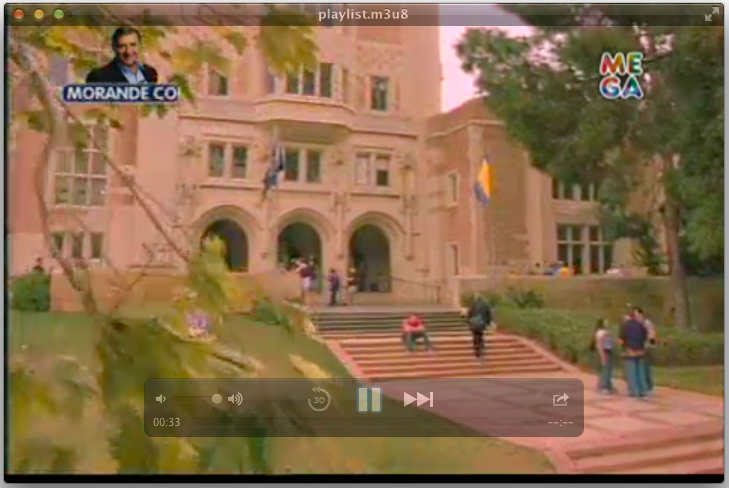
\includegraphics[scale=0.3]{imgs/qt-mega.png} & 
	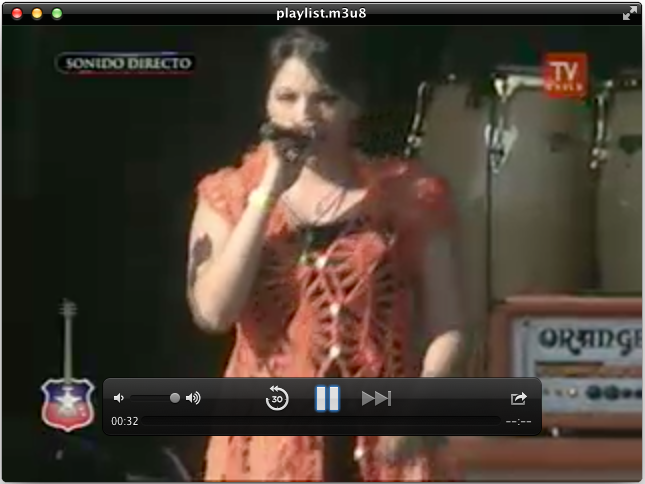
\includegraphics[scale=0.3]{imgs/qt-tvn.png} \\
	\end{tabular}
	\caption{Captura de Quicktime reproduciendo lista de reproducción a través de un URL.}
	\label{qt-tvn-mega}
\end{figure}

Utilizando \textbf{Wireshark} se observaron los datos entregados al cliente desde el servidor como \textit{\textbf{cookies}} indicadas en \ref{subsec:cookies}.

\begin{figure}[H]
	\centering
\begin{lstlisting}
HTTP/1.1 200 OK
Server: nginx/1.2.0
Date: Sat, 24 Nov 2012 18:06:10 GMT
Content-Type: application/vnd.apple.mpegurl
Transfer-Encoding: chunked
Connection: keep-alive
Keep-Alive: timeout=20
X-Powered-By: PHP/5.3.15-1~dotdeb.0
Set-Cookie: stream=tvn
Set-Cookie: t0=1353186024
Set-Cookie: tp=1353780370
Set-Cookie: ti=1353186033
Set-Cookie: tl=1353186085
Set-Cookie: si=1
Set-Cookie: sf=6

#EXTM3U
#EXT-X-TARGETDURATION:10
#EXT-X-PROGRAM-DATE-TIME:2012-11-17T18:00:33-03:00
#EXT-X-VERSION:3
#EXT-X-MEDIA-SEQUENCE:1
#EXTINF:13,
http://ssdemo.altavoz.net/streams/tvn/tvn_1353186033.ts
#EXTINF:10,
http://ssdemo.altavoz.net/streams/tvn/tvn_1353186043.ts
#EXTINF:9,
http://ssdemo.altavoz.net/streams/tvn/tvn_1353186052.ts
#EXTINF:12,
http://ssdemo.altavoz.net/streams/tvn/tvn_1353186063.ts
#EXTINF:7,
http://ssdemo.altavoz.net/streams/tvn/tvn_1353186070.ts
#EXTINF:13,
http://ssdemo.altavoz.net/streams/tvn/tvn_1353186085.ts
\end{lstlisting}
\caption{Información HTTP entregada por servidor Web}
\label{lst:setcookies}
\end{figure}

De la figura \ref{lst:setcookies} se puede observar que el servidor web Ngnix\ref{bib:ngnix-homepage} entrega en la cabecera HTTP las intrucciones Set-Cookie con los valores descritos en \ref{subsec:cookies}. \\

En la siguiente conexión con el servidor, se ajustaran los valores de las \textit{cookies} acorde al contenido de la lista de reproducción entregada. Como se describió anteriormente las \textit{cookies} no son manejados por la aplicación cliente, ya que el sistema operativo iOS se encarga de manejar los valores de estas.\\

En la figura \ref{lst:sequence2} se puede observar que los nuevos valores de cookies son ajustados por el servidor para la lista de reproducción acorde a la segunda secuencia del stream.

\begin{figure}[H]
	\centering
\begin{lstlisting}
HTTP/1.1 200 OK
Server: nginx/1.2.0
Date: Sat, 24 Nov 2012 18:06:25 GMT
Content-Type: application/vnd.apple.mpegurl
Transfer-Encoding: chunked
Connection: keep-alive
Keep-Alive: timeout=20
X-Powered-By: PHP/5.3.15-1~dotdeb.0
Set-Cookie: stream=tvn
Set-Cookie: tp=1353780385
Set-Cookie: ti=1353186043
Set-Cookie: tl=1353186093
Set-Cookie: si=2
Set-Cookie: sf=7

#EXTM3U
#EXT-X-TARGETDURATION:10
#EXT-X-PROGRAM-DATE-TIME:2012-11-17T18:00:43-03:00
#EXT-X-VERSION:3
#EXT-X-MEDIA-SEQUENCE:2
(...)
\end{lstlisting}
\caption{Información HTTP entregada por servidor Web con la lista actualizada para secuencia 2}
\label{lst:sequence2}
\end{figure}



%http://ssdemo.altavoz.net/playlist/playlist.m3u8?s=tvn&t=1353186024&c=0
%http://ssdemo.altavoz.net/playlist/playlist.m3u8?s=video1&t=1353186024&c=0

%escribir en consola el URL, probarlo en quicktime, vlc, navegador, app, wireshark para ver cookies

\section{Proceso corriendo en fondo} % background

Debido a que se utiliza el protocolo HTTP Live Streaming de forma que entregue información en vivo, la instancia de AVPlayer se mantiene realizando peticiones por nuevas listas de reproducción a medida que pase el tiempo, sin importar que la reproducción se encuentre \textbf{pausada} o que la aplicación esté corriendo en el \textbf{fondo} (\textit{background}).\\

Se encontró un problema al interrumpir la reproducción. Sea cual sea el motivo, por ejemplo recibir una llamada telefónica, el sistema iOS envía la aplicación cliente a background pausando la reproducción. Al volver despues de la interrupción la aplicación retoma la reproducción, sin embargo el tiempo que ha pasado implica en  listas de reproducción distintas a la que se estaba viendo.\\

La solución fue establecer una marca de tiempo de 30 segundos, acordes a la ventana de transmisión de la lista, asociada a la instrucción de pausa y reproducción del reproductor, que además es llamada por el botón \textit{Play/Pause} en la interfaz gráfica.\\

Al enviar la aplicación a background se guarda la \textbf{fecha del contenido} del stream y el momento en el cual se ha pausado.
Al volver a \textit{foreground} se activa el método para reanudar la reproducción donde se compara el momento de pausa guardado y el actual. Si esta diferencia es mayor a 30 segundos, se realiza una nueva llamada al servidor mediante URL. Sin embargo cuando la diferencia es menor, se reanuda la reproducción debido a que la fecha del contenido del stream aun se encuentra dentro del rango en la lista que posee la instancia de AVPlayer.\\

El valor de 30 segundos se debe una lista de reproducción con mínimo 3 segmentos de 10 segundos.\\

El problema encontrado se obtuvo gracias a la depuración de la aplicación ejecutandose en un dispositivo iOS (iPhone). Se revisó el valor del \textbf{rango de reproducción} a través de notificaciones por cambios (página \pageref{item:seekableTimeRanges}). A pesar que la reproducción se pausaba o la aplicación se mandaba a background el rango se mantenia en aumento.

%escribir en consola los seekable time ranges, poner pausa background y al retomar reproducir, se notó que avanzaba la lista de iguañl forma. se arregó guardando la fecha al momento de poner pausa. que se llamaba al irse a background.

\section{Cambio de ancho de banda}

El cambio de ancho de banda se revisó mediante Wireshark y modificando el valor de la cadena de consulta \textbf{c} entre 0 (WiFi) y 1 (red celular) en el URL.\\ 

Por ejemplo: \url{http://ssdemo.altavoz.net/playlist/playlist.m3u8?s=tvn&t=1353186024&c=0}
La respuesta fue rastreada obteniendo una lista de reproducción:

\begin{figure}[H]
	\centering
\begin{lstlisting}
#EXTM3U
#EXT-X-STREAM-INF:PROGRAM-ID=1,BANDWIDTH=320000
stream.m3u8?s=tvn&t=1353186024
#EXT-X-STREAM-INF:PROGRAM-ID=1,BANDWIDTH=65000
stream.m3u8?s=tvn&a=1&t=1353186024
\end{lstlisting}
\caption{Lista de reproducción resultante de una petición al servidor con parámetro \textbf{c = 0}}
\label{lst:playlistc0}
\end{figure}

\begin{figure}[H]
	\centering
\begin{lstlisting}
#EXTM3U
#EXT-X-STREAM-INF:PROGRAM-ID=1,BANDWIDTH=65000
stream.m3u8?s=tvn&a=1&t=1353186024
#EXT-X-STREAM-INF:PROGRAM-ID=1,BANDWIDTH=320000
stream.m3u8?s=tvn&t=1353186024
\end{lstlisting}
\caption{Lista de reproducción resultante de una petición al servidor con parámetro \textbf{c = 1}}
\label{lst:playlistc1}
\end{figure}

En el caso de ajustar el valor a 1, la lista de reproducción invierte la prioridad de las variantes del stream, priorizando el enlace que posee sólo audio para un ancho de banda de \textbf{65kbps}. \ref{lst:playlistc1}

%se especifica requerimiento a la empresa, se modifica el dispatcher con lista de variantes, se revisa en wireshark.
%luego se utiliza la herramienta network link conditioner para modificar el BW en plena transmisión, revisar wireshark cuando cambia y ver en la misma app.
%Luego se prueba con iPhone cambiando entre wifi y 3g

  \subsection{WiFi}
  se agrega campo en el URL para priorizar distintas variantes, con wifi video, 3g audio.
  explicar que parte con el video, mostrar 2 imagenes emparejadas.
  \subsection{3G}
  con 3g, imagen de que muestra el audio primero.
\section{Cambio de transmisión mediante Twitter}
- se revisa usando safari desktop con script que incluye player

  \subsection{Dentro de la aplicación}
	- debug viendo el cambio de tranmisión, URL generado y definiendo el mismo canal. manejo en caso de tweet sin enlace
	se genera notificación interna con los componentes. ver que cambia el stream.
  \subsection{Scheme registrado en iOS}
	- clientes de twitter en iPhone, twitter y Tweetbot, debug en el método e imprimir en consola la app que lo lanzó.  
	- debug con app en background
	- debug con app cerrada y a la espera que parta por otra aplicación
	explicar que se detuvo la carga del stream cuando está cerrada y que se espera una notificacion de la carga de la UI antes de cargar el stream.
  
\section{Enlaces Twitter en otros dispositivos}
	pantallazos de páginas de error, el por qué y cómo se entregan según el script, no se revisa internet explorer porque se utilizaron navegadores compatibles con OS X.
	
  \subsection{PC Escritorio}
    \subsubsection{Chrome}
    chrome no es compatible con hls
    foto
    \subsubsection{Safari}
    safari muestra un player html5
    foto del player
    \subsubsection{Firefox}
    firefox no es compatible
    foto
    \subsubsection{Opera}
    opera tampoco
    foto
  \subsection{Android y otros móviles incompatibles}
  pantallazo del cell de la esperanza
  explicar que tampoco es compatible con HLS, por lo menos 2.3, 4.0 ICS en adelante es compatible, pero para reproducir el stream se debe desarrollar una aplicación cliente similar a la hecha en iOS
\section{Comparación con SocialStream Flash}
mostrar player original de eduardo, la diferencia de la linea de tiempo, el salto de tiempo, la exactitud y que no es tan exacto porque los segmentos son de 10 segundos

la linea de tiempo difiere con una representación gráfica, se utilizó el control de fecha para simplificar el punto a elegir, además la linea de tiempo precisa de mouse over para mostrar datos y en el caso táctil difiere mucho.


